%%%%%%%%%%%%%%%%%%%%%%%%%%%%%%%%%%%%%%%%%%%%%%%%%%%%%%%%%%%%%%%%%%%%%%%%%%%%%%%%%%
\begin{frame}[fragile]\frametitle{}
\begin{center}
{\Large Conditionals}
\end{center}
\end{frame}

%%%%%%%%%%%%%%%%%%%%%%%%%%%%%%%%%%%%%%%%%%%%%%%%%%%%%%%%%%%%%%%%%%%%%%%%%%%%%%%%%%%
\begin{frame}[fragile]\frametitle{Conditionals}
What can we deduce from the following text:
\begin{lstlisting}
If it rains tomorrow, I will tidy up the cellar. After this I will paint the walls. If there is some time left, I will do my tax declaration. Otherwise, I will go swimming. In the evening, I will go to the cinema with my wife!
\end{lstlisting}
\end{frame}

%%%%%%%%%%%%%%%%%%%%%%%%%%%%%%%%%%%%%%%%%%%%%%%%%%%%%%%%%%%%%%%%%%%%%%%%%%%%%%%%%%%
\begin{frame}[fragile]\frametitle{Conditionals}
  \begin{columns}[c]
    \begin{column}{0.5\linewidth}
\begin{lstlisting}
If it rains tomorrow, I will do the following:
    - tidy up the cellar 
    - paint the walls
    - If there is some time left, I will 
          - do my tax declaration
Otherwise, I will do the following:
    - go swimming
go to the cinema with my wife in the evening
\end{lstlisting}
      \end{column}
    \begin{column}{0.5\linewidth}
    \begin{center}
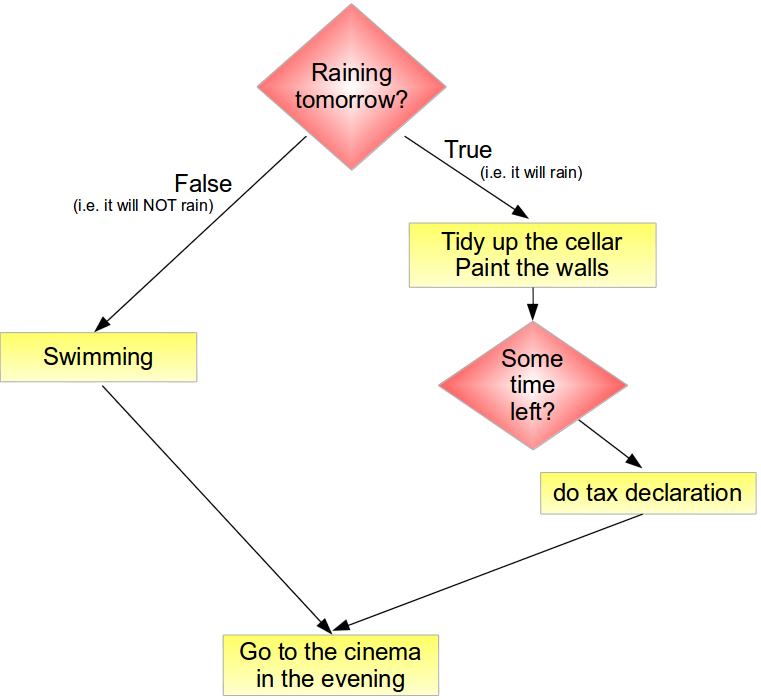
\includegraphics[width=\linewidth,keepaspectratio]{boxes8}
\end{center}
        \end{column}
  \end{columns}
\end{frame}

%%%%%%%%%%%%%%%%%%%%%%%%%%%%%%%%%%%%%%%%%%%%%%%%%%%%%%%%%%%%%%%%%%%%%%%%%%%%%%%%%%%
\begin{frame}[fragile]\frametitle{Conditionals}
  \begin{columns}[c]
    \begin{column}{0.5\linewidth}
    C:
\begin{lstlisting}
if (raining_tomorrow) {
    tidy_up_the_cellar(); 
    paint_the_walls();
    if (time_left) 
          do_taxes();
} else
    enjoy_swimming();
    go_cinema();
\end{lstlisting}
      \end{column}
    \begin{column}{0.5\linewidth}
    Python:
    \begin{lstlisting}
if raining_tomorrow:
    tidy_up_the_cellar() 
    paint_the_walls()
    if time_left: 
          do_taxes()
else:
    enjoy_swimming()
go_cinema()
\end{lstlisting}
        \end{column}
  \end{columns}
\end{frame}

%%%%%%%%%%%%%%%%%%%%%%%%%%%%%%%%%%%%%%%%%%%%%%%%%%%%%%%%%%%%%%%%%%%%%%%%%%%%%%%%%%%
\begin{frame}[fragile]\frametitle{Conditionals}
  Conditional execution uses the \texttt{if} statement:
\begin{lstlisting}
if expr:
  # indented block
elif  other-expr:
  # indented block
else:
  # executed if none of the above matched
\end{lstlisting}

The \texttt{elif} can be repeated, with different conditions, or left out entirely.
Also the \texttt{else} clause is optional.
 

Where's the `end if'?
There's no `end if': indentation delimits blocks!

\end{frame}

%%%%%%%%%%%%%%%%%%%%%%%%%%%%%%%%%%%%%%%%%%%%%%%%%%%%%%%%%%%%%%%%%%%%%%%%%%%%%%%%%%%
\begin{frame}[fragile]\frametitle{Boolean expressions}
A boolean expression is an expression that is either true or false.
\begin{lstlisting}
>>> 5 == 5
True
>>> 5 == 6
False
\end{lstlisting}
True and False are special values that belong to the class bool; they are not
strings:
\begin{lstlisting}
>>> type(True)
<class 'bool'>
>>> type(False)
<class 'bool'>
\end{lstlisting}
\end{frame}

%%%%%%%%%%%%%%%%%%%%%%%%%%%%%%%%%%%%%%%%%%%%%%%%%%%%%%%%%%%%%%%%%%%%%%%%%%%%%%%%%%%
\begin{frame}[fragile]\frametitle{Comparison operators}
== operator is one of the comparison operators; others are:
\begin{lstlisting}
x != y # x is not equal to y
x > y # x is greater than y
x < y # x is less than y
x >= y # x is greater than or equal to y
x <= y # x is less than or equal to y
x is y # x is the same as y
x is not y # x is not the same as y
\end{lstlisting}
\end{frame}

%%%%%%%%%%%%%%%%%%%%%%%%%%%%%%%%%%%%%%%%%%%%%%%%%%%%%%%%%%%%%%%%%%%%%%%%%%%%%%%%%%%
\begin{frame}[fragile]\frametitle{Logical operators}
\begin{itemize}
\item There are three logical operators: and, or, and not. 
\item \lstinline|x > 0 and x < 10| is true only if x is greater than 0 and less than 10.
\item \lstinline|n%2 == 0 or n%3 == 0| is true if either of the conditions is true, that is, if the number is divisible by 2 or 3.
%\item Finally, the not operator negates a boolean expression, so not \lstinline|(x > y)| is true if
%\lstinline|x > y| is false; that is, if x is less than or equal to y.
\end{itemize}
\end{frame}



%%%%%%%%%%%%%%%%%%%%%%%%%%%%%%%%%%%%%%%%%%%%%%%%%%%%%%%%%%%%%%%%%%%%%%%%%%%%%%%%%%%
\begin{frame}[fragile]\frametitle{Quiz: Find Largest}
Python program to find the largest number among the three input numbers
\begin{lstlisting}
num1 = 10
num2 = 14
num3 = 12

# uncomment following lines to take three numbers from user
#num1 = float(input("Enter first number: "))
#num2 = float(input("Enter second number: "))
#num3 = float(input("Enter third number: "))

\end{lstlisting}
\end{frame}


%%%%%%%%%%%%%%%%%%%%%%%%%%%%%%%%%%%%%%%%%%%%%%%%%%%%%%%%%%%%%%%%%%%%%%%%%%%%%%%%%%%
\begin{frame}[fragile]\frametitle{Solution: Find Largest}
\begin{lstlisting}

if (num1 >= num2) and (num1 >= num3):
   largest = num1
elif (num2 >= num1) and (num2 >= num3):
   largest = num2
else:
   largest = num3

print("The largest number between",num1,",",num2,"and",num3,"is",largest)
\end{lstlisting}
\end{frame}


%%%%%%%%%%%%%%%%%%%%%%%%%%%%%%%%%%%%%%%%%%%%%%%%%%%%%%%%%%%%%%%%%%%%%%%%%%%%%%%%%%%
\begin{frame}[fragile]\frametitle{Exercises}
\begin{itemize}
\item Write a Python program to get the difference between a given number and 17, if the number is greater than 17 return double the absolute difference.
\item Write a Python program to calculate the sum of three given numbers, if the values are equal then return thrice of their sum
\item Write a Python program to sum of two given integers. However, if the sum is between 15 to 20 it will return 20.
\end{itemize}
\end{frame}



%%%%%%%%%%%%%%%%%%%%%%%%%%%%%%%%%%%%%%%%%%%%%%%%%%%%%%%%%%%%%%%%%%%%%%%%%%%%%%%%%%%
\begin{frame}[fragile]\frametitle{switch/case}
  \begin{itemize}
\item There is no such statement in Python.
\item Conditional execution uses the \texttt{if} statement
\end{itemize}

\textbf{Advance:}

   It can be implemented efficiently with a dictionary of functions:
\begin{lstlisting}
result = {
	`a': lambda x: x * 5,
	'b': lambda x: x + 7,
	'c': lambda x: x - 2
}
result['b'](10)
\end{lstlisting}

\end{frame}

%%%%%%%%%%%%%%%%%%%%%%%%%%%%%%%%%%%%%%%%%%%%%%%%%%%%%%%%%%%%%%%%%%%%%%%%%%%%%%%%%%%
\begin{frame}[fragile]\frametitle{Exercises}
Rewrite your pay computation to give the employee 1.5 times the
hourly rate for hours worked above 40 hours.
\begin{lstlisting}
Enter Hours: 45
Enter Rate: 10
Pay: 475.0
\end{lstlisting}
Write a program to prompt for a score between 0.0 and 1.0. If the
score is out of range, print an error message. If the score is between 0.0 and 1.0,
print a grade using the following table:
\begin{lstlisting}
Score Grade
>= 0.9 A
>= 0.8 B
>= 0.7 C
>= 0.6 D
< 0.6 F
\end{lstlisting}

\end{frame}



